% Chapter 4

\chapter{Extension of Wu et. al.'s algorithm toward dynamic and social navigation} % Main chapter title

\label{Chapter4} % For referencing the chapter elsewhere, use \ref{Chapter4}

\section{Discussion on the original hypotheses in the light of tests with the Pepper robot}

\paragraph{} As eventually our experimental platform is to be a Pepper robot, in the context of the Robocup@Home challenge that emulates a home setting, several hypotheses from the original algorithms have to be reconsidered :

\begin{itemize}
  \item \textbf{Initial knowledge of the environment} is partial, in that all static obstacles (i.e. objects that are not meant to be moved by any actor, like walls or very heavy furniture) have already been mapped. In the context of the Robocup@Home Challenge, participants are allowed to build such a map prior to the actual trials. This hypothesis is actually quite justified since in a home setting, it is very likely that the robot has undergone a configuration phase prior to its daily use, when it is provided with a manually drawn map of the home, or at least allowed to roam about and map the static obstacles. Having a map of static obstacles is very important for standard localization algorithms used in ROS, like \href{http://wiki.ros.org/amcl}{AMCL}, since they use this environment knowledge to compensate for odometry error.
  \item \textbf{Manipulation actions}, for the moment, are to be limited to pushes in a perpendicular direction to the obstacle's side being pushed. Given the many problematics related to grasping objects (e.g., appropriate positioning of the robot joints, keeping the robot balanced, ...), it is best for a first iteration not to dwell on these.
  \item \textbf{Manipulation poses} are a key concept of manipulating obstacles, as we have shown in the previous chapter, and in contrary to the original algorithms we will explicitly explain our hypotheses as to them. Experimentations with the Pepper Robot and carboard boxes as movable obstacles have shown that a good first approximation that guarantees quasi-systematic push manipulation successes are poses situated at the middle of the object's sides. This is, of course, supposing that we are only considering light objects with negligible friction against the ground, and with no other cinematic constraint than a plan-plan link between one of the obstacle's faces and the ground (a perfect plane).
  % TODO Add figures showing:
  % - Pepper pushing carboard box and chair, noting the difference of trajectory
  \item \textbf{Manipulation cost} A constant $pushCost$ has been used in the previously shown algorithm to allow weighting of the manipulation action in regard to a simple move action. Semantically, it makes more sense that this constant be related to the object (the difficulty of moving a specific object depending mainly of its physical properties), so we will store it as an obstacle attribute.
  \item \textbf{Manipulation possibility check} Checking whether a manipulation is possible or not is the same as checking whether the area covered by the robot and the obstacle as they move together is not in intersection with any other obstacle. As we limit our action set to pushes in a specific direction, this area can be defined of the convex hull containing both the robot's and the obstacle's polygonal representation at their initial and final position. According to the existing litterature, we will call this the "safe-swept area" if no other obstacle is in intersection with it. In the following pseudocode, this is done by the "GET-SAFE-SWEPT-AREA" method, which returns null if any obstacle is in intersection with the manipulation area. This area is saved as part of the plan so that when the plan is being executed, checking for a collision is as simple as checking if an obstacle appeared in this area.
  \item \textbf{Obstacle discovery} As the robot approaches obstacles, their geometrical representation is updated according to what the robot's sensors can see. When executing a plan that includes the manipulation of an obstacle, said obstacle can actually change during the execution of the $c_{1}$ component, which is problematic for the preservation of optimality, since the obstacle's push poses may change (it is defined with a dependency to the side's middle point). Therefore re-evaluation should not only be triggered if a new obstacle intersects with the current optimal plan, but also if the current optimal plan includes the manipulation of an obstacle and if said obstacle has changed in a way that makes the originally targeted $pushPose$ unavailable.
\end{itemize}

\paragraph{}\label{check_opening_solution} Below, we propose, a way for restoring the optimality, assuming we are under the hypothesis of sole translations in a single direction:

\paragraph{} A new opening detection is defined by the disparition of at least one blocking area thanks to the considered manipulation. A new opening is never detected if :

\begin{itemize}
  \item Not a single blocking area disappears thanks to the considered manipulation, because the blocking areas do not vary enough or at all ("corridor" case),
  \item There are no blocking areas to begin with ("open space" case).
\end{itemize}

\begin{figure}[H]
\centering
\begin{subfigure}{.5\textwidth}
  \centering
  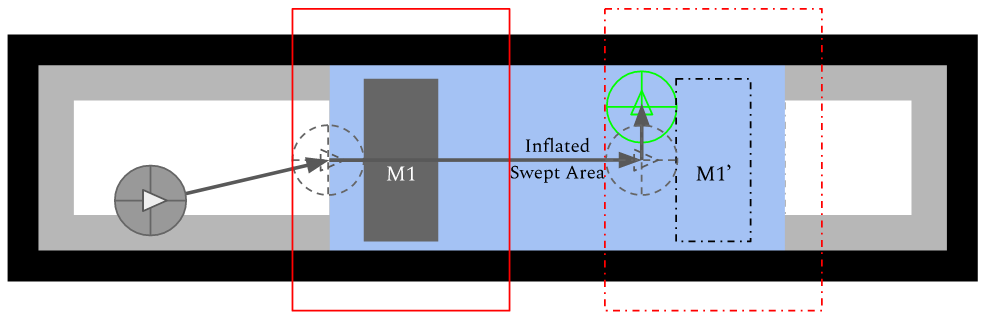
\includegraphics[width=\linewidth]{Figures/Check_New_Opening/corridor_swept.png}
  \caption{"Corridor" case}
  \label{fig:corridor_swept}
\end{subfigure}%
\begin{subfigure}{.5\textwidth}
  \centering
  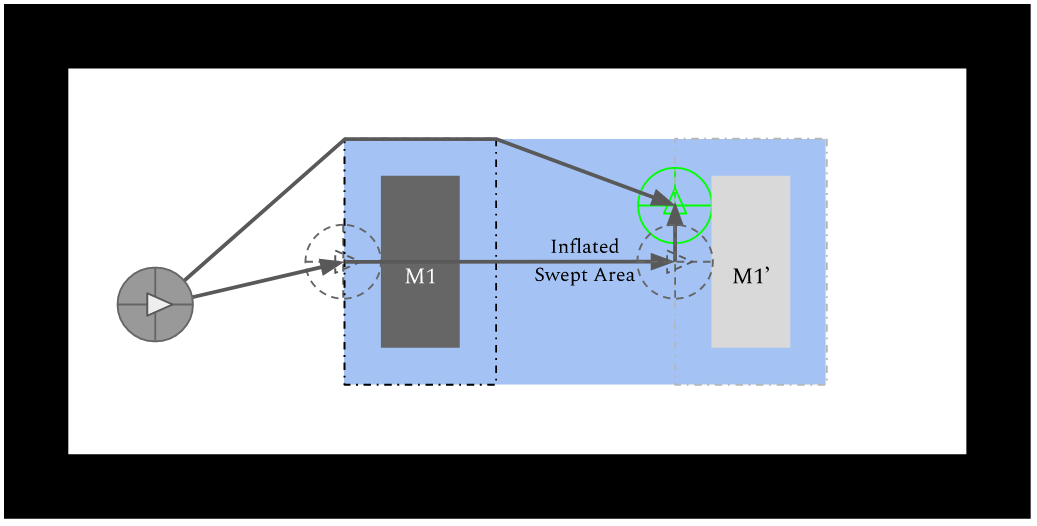
\includegraphics[width=\linewidth]{Figures/Check_New_Opening/openspace_swept.png}
  \caption{"Open space" case}
  \label{fig:openspace_swept}
\end{subfigure}
\caption{Limit cases of the original algorithm with illustration of the "Inflated swept area"}
\label{fig:inflated_swept_area}
\end{figure}

\paragraph{} In both cases, it is only interesting to consider the manipulation if it actually creates any chance of finding a path that has a lower cost than the one that avoids the obstacle. If no new opening is detected, and if, like in the "corridor" case, no path avoiding the obstacle was found, or, like in the "open space" case, a path avoiding the obstacle was found, we should only consider the manipulation if it allows us to push the obstacle through the goal pose; in more precise terms, \textbf{if the goal pose is within the "inflated swept area" and the obstacle in its final position does not intersect with the goal pose}. The inflated swept area is defined as the area covered by the inflated (by the robot's radius) obstacle when moved. In the end, the overall check condition should be :

\paragraph{} \textbf{If} CHECK-NEW-OPENING($I.occGrid$, $o$, $translation$, $BA$) AND $goalPose \in$ GET-INFLATED-SWEPT-AREA($o$, $translation$, $I$) AND $goalPose \not\in o.inflatedArea$


\paragraph{} We have an intuition that these two extra verifications steps are sufficient allow to restore optimality, but this is no proper demonstration. Since performance is not the main focus of our work here, but optimality is, we will prefer not to use the opening check optimization step in our following algorithms propositions, and postpone a proof to later work.

\paragraph{Note on \textbf{continue}}\label{continue_note} The \textbf{continue} statement returns the control to the beginning of the loop, and simply won't execute any of the remaining statements in the current iteration of the loop. This is done because a plan with a manipulation cannot exist without an empty $c_{1}$ component.

\paragraph{Note on COPY}\label{copy_note} Here, $p_{opt}.o$ is a copy of object $o$, and not the same object, so that when $o$ is updated because of the call to UPDATE-FROM-NEW-INFORMATION() on $I$, we can compare the difference between the two. We do the same for $p_{opt}.pushPose$ for the same reason. This allows us to trigger re-evaluation if the obstacle's push poses change and the one the robot aimed for no longer exists.

\paragraph{Note on [] and $\neq$}\label{operators_note} Here, the [] operator is used as a short handle for "get the obstacle that corresponds in $\mathcal{O}$ that corresponds to the saved obstacle $p_{opt}.o$. The $\neq$ operator checks if the two states of the obstacle are the same or not (i.e, if the obstacle changed).

\paragraph{Note on the use of $\bigcap$}\label{area_intersect_note} The notation $\bigcap$ means here that we check for possible collisions between the swept area and any obstacle, since they may have changed.

\paragraph{Note on saving $translation$ in $p_{opt}$}\label{translation_note} The $translation$ necessary for manipulating the obstacle is saved to easily recompute the safe swept area when the obstacle changes.

\begin{algorithm}[H]

  \caption{Execution loop taking our hypotheses into account.}

  \label{alg:03-custom-basicmods-makeandexecuteplan}

  \begin{algorithmic}[1]

    \Procedure{MAKE-AND-EXECUTE-PLAN}{$R_{init}$, $R_{goal}$, $I_{init}$}

      \State \dots \label{lst:line:initbis1} \Comment{Initialization (lines \ref{lst:line:init1} to \ref{lst:line:init2} in Algorithm \ref{alg:02-levihn-makeandexecuteplan})}

      \State \hlgreen{$I \gets I_{init}$}

      \State $p_{opt}.components \gets [$\hlgreen{$A$*}($R_{init}$, $R_{goal}$, $I$)]
      \State $p_{opt}.cost \gets |p_{opt}| * moveCost$ \label{lst:line:initbis2}

      \While{$R \neq R_{goal}$}

        \State UPDATE-FROM-NEW-INFORMATION($I$) \label{lst:line:knowledge1}

        \If{$I$.freeSpaceCreated}
          \State $minCostL \gets \emptyset$
        \EndIf

        \State $\mathcal{O}_{new} \gets \mathcal{O}_{new} \bigcup I.newObstacles$

        \State $\mathcal{O} \gets I.allObstacles$

        \State $isPathFree \gets p_{opt} \bigcap \mathcal{O}_{new} \neq \emptyset$

        \State \hlgreen{$isPushPoseValid \gets True$} \label{lst:line:validity1}
        \State \hlgreen{$isManipSafe \gets True$}
        \State \hlgreen{$isObstacleSame \gets True$}
        \If{\hlgreen{$p_{opt}.o$ exists}} \Comment{If $p_{opt}$ includes the manipulation of an obstacle.}
          \State \hlgreen{$isObstacleSame \gets \mathcal{O}[p_{opt}.o] = p_{opt}.o$} \Comment{\nameref{operators_note}}
          \If{\hlgreen{\textbf{not} $isObstacleSame$}}
            \State \hlgreen{$p_{opt}.o \gets \mathcal{O}[p_{opt}.o.id]$} \Comment{Update the copy.}
            \State \hlgreen{$p_{opt}.safeSweptArea \gets$ GET-SAFE-SWEPT-AREA($p_{opt}.o$, $p_{opt}.translation$, $I$)}
            \If{\hlgreen{$p_{opt}.pushPose \not\in p_{opt}.o.pushPoses$}}
              \State \hlgreen{$isPushPoseValid \gets False$}
            \EndIf
          \EndIf
          \If{\hlgreen{$p_{opt}.safeSweptArea \bigcap \mathcal{O} \neq \emptyset$}} \Comment{\nameref{area_intersect_note}}
            \State \hlgreen{$isManipSafe \gets False$}
          \EndIf
        \EndIf \label{lst:line:knowledge2} \label{lst:line:validity2}

        \If{\textbf{not}($isPathFree$ AND $isManipSuccess$ \hlgreen{AND $isManipSafe$ AND $isPushPoseValid$})}
          \State $p_{opt}.components \gets$ [\hlgreen{$A$*}($R$, $R_{goal}$, $I$)]
          \State $p_{opt}.cost \gets |p_{opt}| * moveCost$
          \State MAKE-PLAN($R$, $R_{goal}$, $I$, $\mathcal{O}$, $blockedObsL$, $p_{opt}$, $euCostL$, $minCostL$)
          \State $\mathcal{O}_{new} \gets \emptyset$
        \EndIf

        \State \dots \Comment{Execution (lines \ref{lst:line:exec1} to \ref{lst:line:exec2} in Algorithm \ref{alg:02-levihn-makeandexecuteplan})}

      \EndWhile

      \State \textbf{return} $True$

    \EndProcedure

  \end{algorithmic}
\end{algorithm}


\begin{algorithm}[H]

  \caption{Obstacle evaluation subroutine taking our hypotheses into account.}

  \label{alg:03-custom-basicmods-planforobstacle}

  \begin{algorithmic}[1]

    \Procedure{PLAN-FOR-OBSTACLE}{$o$, $p_{opt}$, $I$, $R$, $R_{goal}$, $blockedObsL$}

      \If{$o \in blockedObsL$} \label{lst:line:initobs1}
        \State \textbf{return} null
      \EndIf \label{lst:line:initobs2}

      \State $P_{o,d}$ $\gets \emptyset$
      % \State $BA \gets null$

      \For{\hlgreen{each $pushPose$ in $o.pushPoses$}}
        \State \hlgreen{$pushUnit \gets (cos(pushPose.yaw), sin(pushPose.yaw))$} \label{lst:line:loop1} \Comment{Unit vector for push direction}

        \State \hlgreen{$c_{1} \gets A$*($R$, $pushPose$, $I$)} \Comment{$c_{1}$ is computed for each push pose}

        \If{$c_{1} = \emptyset$}
          \State \hlgreen{\textbf{continue}} \Comment{\nameref{continue_note}}
        \EndIf

        \State $seq \gets 1$

        \State \hlgreen{$translation \gets pushUnit * onePushDist * seq$} \Comment{onePushDist is a distance constant}

        \State \hlgreen{$safeSweptArea \gets $GET-SAFE-SWEPT-AREA($o$, $translation$, $I$)}

        \State $oSimPose \gets $\hlgreen{$pushPose + translation$} \label{lst:line:loop2}

        \State $c_{3_{(Est)}} \gets \{oSimPose, R_{goal}\}$

        \State $C_{est} \gets (|c_{1}| + |c_{3_{(Est)}}|) * moveCost + $\hlgreen{$|translation| * o.pushCost$}

        \While{$C_{est}$ $ \leq p_{opt}.cost$ AND \hlgreen{$safeSweptArea \neq$ null}}

          % \If{CHECK-NEW-OPENING($I.occGrid$, $o$, $translation$, $BA$)}
            \State $c_{2} \gets \{$\hlgreen{$pushPose$}$, oSimPose\}$
            \State \hlgreen{$c_{3} \gets A$*($oSimPose$, $R_{goal}$, $I.withSimulatedObstacleMove$)}
            \If{$c_{3} \neq \emptyset$}
              \State $p.components \gets$ [$c_{1}$, $c_{2}$, $c_{3}$]
              \State $p.cost \gets (|c_{1}| + |c_{3}|) * moveCost + |c_{2}| * $\hlgreen{$o.pushCost$}
              \State $p.minCost \gets |c_{2}| * $\hlgreen{$o.pushCost$}$ + |c_{3}| * moveCost$
              \State $p.o \gets$ \hlgreen{COPY($o$)} \label{lst:line:ovaraffec1} \Comment{\nameref{copy_note}}
              \State \hlgreen{$p.translation \gets translation$} \Comment{\nameref{translation_note}}
              \State \hlgreen{$p.safeSweptArea \gets safeSweptArea$}
              \State $P_{o,d} \gets P_{o,d} \bigcup \{p\}$
              \If{$p.cost < p_{opt}.cost$}
                \State $p_{opt} \gets p$
              \EndIf \label{lst:line:ovaraffec2}
            \EndIf
          % \EndIf

          \State $seq \gets seq + 1$ \label{lst:line:loopvarup1}

          \State \hlgreen{$translation \gets pushUnit * onePushDist * seq$}

          \State \hlgreen{$safeSweptArea \gets $GET-SAFE-SWEPT-AREA($o$, $translation$, $I$)}

          \State $oSimPose \gets $\hlgreen{$pushPose + translation$} \label{lst:line:loopvarup2}

          \State $c_{3_{(Est)}} \gets \{oSimPose, R_{goal}\}$

          \State $C_{est} \gets (|c_{1}| + |c_{3_{(Est)}}|) * moveCost + $\hlgreen{$|translation| * o.pushCost$}

        \EndWhile

      \EndFor

    \State \textbf{return} $p \in P_{o,d}$ with minimal $p.cost$ or null if $P_{o,d} = \emptyset$

    \EndProcedure

  \end{algorithmic}
\end{algorithm}


\section{Social awareness through risk consideration}

\paragraph{} As shown in Chapter \ref{Chapter2}, to the best of our knowledge, the current NAMO litterature has never covered the idea of socially-aware navigation. Then, we must ask: what makes the action of moving an obstacle socially-aware or not ?

\paragraph{} The first thing that comes to mind would be to consider that some objects are better not be moved because:

\begin{itemize}
  \item they are too fragile (e.g. flower pot),
  \item they have a high value in the human’s eye (e.g. a costly vase)
  \item they might cause the robot to break if it fails to move them properly (i.e. heavy or unstable objects)
  \item they are not supposed to be moved (i.e. exhibited objects)
\end{itemize}

\paragraph{} Thus comes the notion of risk, either to the robot or to the manipulated objects. To mitigate this risk, we propose to modify our base algorithm so that an obstacle is not to be moved unless identified as belonging to a provided whitelist of "movable" obstacles.

% TODO Add a link to research by Christian Wolf on object detection (go to Lyontech website to find it)
% TODO Add handmade figure that shows cases where Pepper mimght detect an obstacle and not
% TODO Add screenshots and figures of obstacle detection from video of Lyontech team to show that obstacle is not necessarily identified at the same time it is detected
\paragraph{} This identification of the obstacle's nature is to be done through computer vision, since it is one of the most efficient and most common ways to detect specific objects, by using trained neural networks for example. However, robots come with all sort of sensors to detect obstacles: laser range finders, RGB(D) cameras, sonars, ... And often, as with Pepper, their fields of vision do not perfectly overlap: typically, an obstacle may be detected by the laser range finders or the sonars, but not be within the field of vision of the RGB(D) camera, because it is in its blind spot or simply too close or too far away. This creates a situation where the robot knows an obstacle is there, but cannot definitely categorize it as "movable" or "unmovable" since it is not in the camera's field of vision.

\paragraph{} Then, it means that the algorithm must be adapted not only to manage the fact that an object should be considered for manipulation if and only if it is deemed "movable", but also to eventually adapt the robot's trajectory \textbf{in an optimal way} so that an "unidentified" / "potentially movable" object can be identified with certainty before engaging with the manipulation procedure.

\paragraph{} For that, when we evaluate an obstacle, we first check whether the obstacle has already been identified or not. If it has been identified as "movable", the algorithm does not change. If it has been identified as "unmovable", the obstacle evaluation routine simply stops before actually evaluating. And finally, if the evaluated obstacle is "unidentified":

% TODO add 2d figure representing the robot and the shape of its field of vision with the appropriate parameters
\begin{itemize}
  \item The $c_{1}$ plan component that goes from the current robot pose to the push pose is evaluated,
  \item If a pose comprised in the computed $c_{1}$ component allows the camera field of vision (which is condidered to be cutoff cone) to encompass the obstacle's currently known geometry, keep the precomputed $c_{1}$ component,
  \item Else we must find a path shortest path component $c_{0}$ from the current robot pose to an "observation pose" where we know we can identify the obstacle as "movable" or not with certainty and recompute $c_{1}$ as the path from this "observation pose" to the push pose.
  \item The observation poses are updated in the same way that push poses are: automatically, whenever an obstacle is updated. These poses are situated at every grid point for which the field of vision of the robot sensor(s) dedicated to obstacle recognition covers the entire known obstacle's geometry. Though the presented algorithm is not affected by the representation of the identification sensor's field of vision, in our experimentation, we will consider a single RGB(D) camera, and approximate its field of vision by the difference between a circular sector and a disk of same center, coincident with the robot's center, which is an acceptable representation for the Pepper robot. The circular sector has a radius $r_{max}$, central angle $\theta$ and is equally partitioned around the robot's orientation direction line. The disk has a radius $r_{min}$.
  \item To find $c_{0}$ and $c_{1}$, a heuristic cost defined as the sum of the euclidian distance between the current pose and observation pose, and euclidean distance between observation pose and currently evaluated push pose is computed for every observation pose, and allows to order them in a list $obsPoseL$, sorted by ascending heuristic cost. The list is then traversed until the heuristic cost of the current element is greater than the current optimal cost of $c_{0}$ + $c_{1}$.
\end{itemize}

\begin{algorithm}[H]

  \caption{Execution loop modified for allowing observation.}

  \label{alg:04-custom-observation-makeandexecuteplan}

  \begin{algorithmic}[1]

    \Procedure{MAKE-AND-EXECUTE-PLAN}{$R_{init}$, $R_{goal}$, $I_{init}$}

      \State \dots \Comment{Initialization (lines 2 to 5 in Algorithm \ref{alg:03-custom-basicmods-makeandexecuteplan})}

      \State \hlgreen{$isObservable \gets True$}

      \While{$R \neq R_{goal}$}

        \State UPDATE-FROM-NEW-INFORMATION($I$)

        \State \dots \Comment{Knowledge update and checks (lines 7 to 29 in Algorithm \ref{alg:03-custom-basicmods-makeandexecuteplan})}

        \If{\textbf{not}($isPathFree$ AND $isManipSuccess$ AND $isManipSafe$ AND $isPushPoseValid$ \hlgreen{AND $isObservable$})}
          \State $p_{opt}.components \gets [A$*($R$, $R_{goal}$, $I.occGrid$)]
          \State $p_{opt}.cost \gets |p_{opt}| * moveCost$
          \State MAKE-PLAN($R$, $R_{goal}$, $I$, $\mathcal{O}$, $blockedObsL$, $p_{opt}$, $euCostL$, $minCostL$)
          \State $\mathcal{O}_{new} \gets \emptyset$
        \EndIf

        \If{$p_{opt}.components = \emptyset$}
          \State \textbf{return} $False$
        \EndIf

        \State $isManipSuccess \gets True$
        \State \hlgreen{$isObservable \gets True$}
        \State $R_{next} \gets p_{opt}$.getNextStep()
        \State $c_{next} \gets p_{opt}$.getNextStepComponent()
        \If{\hlgreen{$p_{opt}.o.movableStatus = IS\_MAYBE\_MOVABLE$ AND \textbf{not} $isObstacleSame$ AND ($c_{next} = o_{1}$ OR $c_{next} = c_{1}$)}}
          \State \hlgreen{$fObsPose \gets$ GET-FIRST-PATH-OBSPOSE($p_{opt}.o$, $p_{opt}$.get-$o_{1}$() + $p_{opt}$.get-$c_{1}$(), $I$)}
          \If{\hlgreen{$fObsPose =$ null}}
            \State \hlgreen{$isObservable \gets False$}
            \State \hlgreen{\textbf{continue}}
          \EndIf
        \EndIf
        \State $R_{real} \gets$ ROBOT-GOTO($R_{next}$)
        \If{$c_{next} = c_{2}$ AND $R_{real} \neq R_{next}$}
          \State $isManipSuccess \gets False$
          \State $blockedObsL \gets blockedObsL \bigcup p_{opt}.o$
        \EndIf
        \State $R \gets R_{real}$

      \EndWhile

      \State \textbf{return} $True$

    \EndProcedure

  \end{algorithmic}
\end{algorithm}


\begin{algorithm}[H]

  \caption{Obstacle evaluation subroutine modified for allowing observation.}

  \label{alg:04-custom-observation-planforobstacle}

  \begin{algorithmic}[1]

    \Procedure{PLAN-FOR-OBSTACLE}{$o$, $p_{opt}$, $I$, $R$, $R_{goal}$, $blockedObsL$}

      \If{$o \in blockedObsL$ \hlgreen{OR $o.movableStatus = IS\_NOT\_MOVABLE$}}
        \State \textbf{return} null
      \EndIf

      \State $P_{o,d}$ $\gets \emptyset$
      % \State $BA \gets null$

      \For{each $pushPose$ in $o.pushPoses$}
        \State $pushUnit \gets (cos(pushPose.yaw), sin(pushPose.yaw))$

        \State $c_{1} \gets A$*($R$, $pushPose$, $I$)

        \If{$c_{1} = \emptyset$}
          \State \textbf{continue}
        \EndIf

        %% BEGIN HLGREEN
        \State \hlgreen{$c_{0} \gets \emptyset$}

        \If{\hlgreen{$o.movableStatus = IS\_MAYBE\_MOVABLE$}}

          \State \hlgreen{$obsPose \gets$ GET-FIRST-PATH-OBSPOSE($o$, $c_{1}$, $I$)}

          \If{\hlgreen{$obsPose \neq$ null}}
            \State \hlgreen{$c_{0}, c_{1} \gets c_{1}[c_{1}.firstPose:obsPose], c_{1}[obsPose:c_{1}.lastPose]$}
          \Else
            \State \hlgreen{COMPUTE-O1-C1($o$, $I$, $R$, $pushPose$, $c_{0}$, $c_{1}$)}

            \If{\hlgreen{$c_{0} = \emptyset$ OR $c_{1} = \emptyset$}}
              \State \hlgreen{\textbf{continue}}
            \EndIf
          \EndIf
        \EndIf
        %% STOP HLGREEN

        \State $seq \gets 1$

        \State $translation \gets pushUnit * onePushDist * seq$

        \State $safeSweptArea \gets $GET-SAFE-SWEPT-AREA($o$, $translation$, $I$)

        \State $oSimPose \gets pushPose + translation$

        \State $c_{3_{(Est)}} \gets \{oSimPose, R_{goal}\}$

        \State $C_{est} \gets ($\hlgreen{$(c_{0} \neq \emptyset ? |c_{0}| : 0)$}$ + |c_{1}| + |c_{3_{(Est)}}|) * moveCost + |translation| * o.pushCost$

        \While{$C_{est}$ $ \leq p_{opt}.cost$ AND $safeSweptArea \neq$ null}

          % \If{CHECK-NEW-OPENING($I.occGrid$, $o$, $translation$, $BA$)}
            \State $c_{2} \gets \{pushPose, oSimPose\}$
            \State $c_{3} \gets A$*($oSimPose$, $R_{goal}$, $I.withSimulatedObstacleMove$)
            \If{$c_{3} \neq \emptyset$}
              \State $p.components \gets$ \hlgreen{$c_{0} \neq \emptyset$ ? [$c_{0}$, $c_{1}$, $c_{2}$, $c_{3}$] : [$c_{1}$, $c_{2}$, $c_{3}$]}
              \State $p.cost \gets ($\hlgreen{$(c_{0} \neq \emptyset ? |c_{0}| : 0)$}$ + |c_{1}| + |c_{3}|) * moveCost + |c_{2}| * o.pushCost$
              \State $p.minCost \gets |c_{2}| * o.pushCost + |c_{3}| * moveCost$
              \State \dots \Comment{Affectation of other variables of $p$ (lines \ref{lst:line:ovaraffec1} to \ref{lst:line:ovaraffec2} in Algorithm \ref{alg:03-custom-basicmods-planforobstacle})}
            \EndIf
          % \EndIf

          \State $seq \gets seq + 1$

          \State $translation \gets pushUnit * onePushDist * seq$

          \State $safeSweptArea \gets $GET-SAFE-SWEPT-AREA($o$, $translation$, $I$)

          \State $oSimPose \gets pushPose + translation$

          \State $c_{3_{(Est)}} \gets \{oSimPose, R_{goal}\}$

          \State $C_{est} \gets ($\hlgreen{$(c_{0} \neq \emptyset ? |c_{0}| : 0)$}$ + |c_{1}| + |c_{3_{(Est)}}|) * moveCost + |translation| * o.pushCost$

        \EndWhile

      \EndFor

    \State \textbf{return} $p \in P_{o,d}$ with minimal $p.cost$ or null if $P_{o,d} = \emptyset$

    \EndProcedure

  \end{algorithmic}
\end{algorithm}

\begin{algorithm}[H]

  \caption{Subroutine for getting the first pose in a $path$ that allows identification of $o$, it it exists.}

  \label{alg:04-custom-observation-simple-checkpath}
  
  \begin{algorithmic}[1]

    \Procedure{GET-FIRST-PATH-OBSPOSE}{$o$, $path$, $I$}
      \For{each $pose$ in $path$}
        \If{IS-OBS-IN-FOV-FOR-POSE($o$, $pose$, $I$)}
          \State \textbf{return} $pose$
        \EndIf
      \EndFor
      \State \textbf{return} null
    \EndProcedure
  \end{algorithmic}
\end{algorithm}

\begin{algorithm}[H]

  \caption{Subroutine for computing $c_{0}$ and $c_{1}$ if $c_{1}$ is not already valid.}

  \label{alg:04-custom-observation-simple-compute01c1}

  \begin{algorithmic}[1]

    \Procedure{COMPUTE-C0-C1}{$o$, $I$, $R$, $pushPose$, $c_{0}$, $c_{1}$}
      \State $c_{1} \gets \emptyset$
      \State $totalCost \gets +\infty$

      \For{each $obsPose$ in $o.obsPoses$}
        \State $o \gets A$*($R$, $obsPose$, $I$)
        \State $c \gets A$*($obsPose$, $pushPose$, $I$)
        \State $newTotalCost = |o| + |c|$
        \If{$newTotalCost < +\infty$ AND ($newTotalCost < totalCost$ OR ($newTotalCost = totalCost$ AND $|o| < |c_{0}|$)}
          \State $c_{0} = o$
          \State $c_{1} = c$
          \State $totalCost = |c_{0}| + |c_{1}|$
        \EndIf
      \EndFor
    \EndProcedure

  \end{algorithmic}
\end{algorithm}


\begin{algorithm}[H]

  \caption{Optimized subroutine for computing $c_{0}$ and $c_{1}$ if $c_{1}$ is not already valid.}

  \label{alg:04-custom-observation-optimized-compute01c1}

  \begin{algorithmic}[1]

    \Procedure{OPT-COMPUTE-C0-C1}{$o$, $I$, $R$, $pushPose$, $c_{0}$, $c_{1}$}
      \State $c_{1} \gets \emptyset$
      \State $totalCost \gets +\infty$

      %   % The computation time could be reduced by computing the heuristic
      %   % euclidean cost from current position to obstacle only once and not
      %   % as many times as there are push poses for the obstacle.
      %   % This needs to be added to the calling method and euCostToObsL passed in parameter.
      % \If{$o.movableStatus = IS\_MAYBE\_MOVABLE$}
      %   \State $euCostToObsL \gets \emptyset$
      %   \For{each $obsPose$ in $o.obsPoses$}
      %     \State $euCostToObsL$.insert$(\{obsPose, |{R, obsPose}|\})$
      %   \EndFor
      %
      % \EndIf

      \State $euPosesCostL \gets \emptyset$ \Comment{Sort observation poses by ascending heuristic cost.} \label{lst:line:occ_heur_1}
      \For{each $obsPose$ in $o.obsPoses$}
        \State $euPosesCostL$.insert$(\{obsPose, |{R, obsPose}| + |{obsPose, pushPose}|\})$
      \EndFor \label{lst:line:occ_heur_2}

      \If{$euPosesCostL \neq \emptyset$} \label{lst:line:traverse_eu_1}
        \State $op_{next} \gets euPosesCostL[0]$
        \While{$totalCost \geq op_{next}.cost$ AND $op_{next} \neq$ null}
          \State $c_{0_{cur}} \gets A$*($R$, $op_{next}.obsPose$, $I.occGrid$)
          \State $c_{1_{cur}} \gets A$*($op_{next}.obsPose$, $pushPose$, $I.occGrid$)
          \State $newTotalCost = |c_{0_{cur}}| + |c_{1_{cur}}|$
          \If{$newTotalCost < +\infty$ AND ($newTotalCost < totalCost$ OR ($newTotalCost = totalCost$ AND $|c_{0_{cur}}| < |c_{0}|$)}
            \State $c_{0} = c_{0_{cur}}$
            \State $c_{1} = c_{1_{cur}}$
            \State $totalCost = |c_{0}| + |c_{1}|$
          \EndIf
          \State $op_{next} \gets euPosesCostL$.getNext()
        \EndWhile
      \EndIf \label{lst:line:traverse_eu_2}
    \EndProcedure

  \end{algorithmic}
\end{algorithm}


\section{Social awareness through placement consideration}

\begin{algorithm}[H]

  \caption{Obstacle evaluation subroutine modified for considering placement.}

  \label{alg:05-custom-placement-planforobstacle}

  \begin{algorithmic}[1]

    \Procedure{PLAN-FOR-OBSTACLE}{$o$, $p_{opt}$, $I$, $R$, $R_{goal}$, $blockedObsL$, $occCostGrid$}

      \State \dots \Comment{Initialization (lines \ref{lst:line:initobs1} to \ref{lst:line:initobs2} in Algorithm \ref{alg:03-custom-basicmods-planforobstacle})}

      \For{each $pushPose$ in $o.pushPoses$}
        \State \dots \Comment{Loop initialization (lines \ref{lst:line:loop1} to \ref{lst:line:loop2} in Algorithm \ref{alg:03-custom-basicmods-planforobstacle})}

        \State \hlgreen{$suppC_{M} \gets $GET-OCC-COST(GET-OBS-POINTS($o$, $translation$), $occCostGrid$)}

        \State $c_{3_{(Est)}} \gets \{oSimPose, R_{goal}\}$

        \State $C_{est} \gets (|c_{1}| + |c_{3_{(Est)}}|) * moveCost + |translation| * o.pushCost *$ \hlgreen{$suppC_{M}$}

        \While{$C_{est}$ $ \leq p_{opt}.cost$ AND $safeSweptArea \neq$ null}

          % \If{CHECK-NEW-OPENING($I.occGrid$, $o$, $translation$, $BA$)}
            \State $c_{2} \gets \{pushPose, oSimPose\}$
            \State $c_{3} \gets A$*($oSimPose$, $R_{goal}$, $I.withSimulatedObstacleMove$)
            \If{$c_{3} \neq \emptyset$}
              \State $p.components \gets$ [$c_{1}$, $c_{2}$, $c_{3}$]
              \State $p.cost \gets (|c_{1}| + |c_{3}|) * moveCost + |c_{2}| * o.pushCost *$ \hlgreen{$suppC_{M}$}
              \State $p.minCost \gets |c_{2}| * o.pushCost *$ \hlgreen{$suppC_{M}$} $+ |c_{3}| * moveCost$
              \State \dots \Comment{Affectation of other variables of $p$ (lines \ref{lst:line:ovaraffec1} to \ref{lst:line:ovaraffec2} in Algorithm \ref{alg:03-custom-basicmods-planforobstacle})}
            \EndIf
          % \EndIf

          \State \dots \Comment{Loop variable update (lines \ref{lst:line:loopvarup1} to \ref{lst:line:loopvarup2} in Algorithm \ref{alg:03-custom-basicmods-planforobstacle})}

          \State \hlgreen{$suppC_{M} \gets $GET-OCC-COST(GET-OBS-POINTS($o$, $translation$), $occCostGrid$)}

          \State $c_{3_{(Est)}} \gets \{oSimPose, R_{goal}\}$

          \State $C_{est} \gets (|c_{1}| + |c_{3_{(Est)}}|) * moveCost + |translation| * o.pushCost *$ \hlgreen{$suppC_{M}$}

        \EndWhile

      \EndFor

    \State \textbf{return} $p \in P_{o,d}$ with minimal $p.cost$ or null if $P_{o,d} = \emptyset$

    \EndProcedure

  \end{algorithmic}
\end{algorithm}


\section{Taking dynamic obstacles into account}

\begin{algorithm}[H]

  \caption{Execution loop taking dynamic obstacles into account.}

  \label{alg:06-custom-dynamic-makeandexecuteplan}

  \begin{algorithmic}[1]

    \Procedure{MAKE-AND-EXECUTE-PLAN}{$R_{init}$, $R_{goal}$, $I_{init}$}

      \State \dots \Comment{Initialization (lines \ref{lst:line:initbis1} to \ref{lst:line:initbis2} in Algorithm \ref{alg:03-custom-basicmods-makeandexecuteplan})}

      \State $isBlockingObsMoved \gets False$

      \While{$R \neq R_{goal}$}

        \State UPDATE-FROM-NEW-INFORMATION($I$)

        \If{$I$.freeSpaceCreated}
          \State $minCostL \gets \emptyset$
        \EndIf

        \State $\mathcal{O} \gets I.allObstacles$

        \State $isPathFree \gets p_{opt} \bigcap \mathcal{O} \neq \emptyset$

        \State \hlgreen{$isBlockingObsMoved \gets I.movedObstacles \neq \emptyset$}

        \State \dots \Comment{Plan validity checks (lines \ref{lst:line:validity1} to \ref{lst:line:validity2} in Algorithm \ref{alg:03-custom-basicmods-makeandexecuteplan})}

        \State \hlgreen{$isPlanValid \gets$ ($isPathFree$ AND $isManipSuccess$ AND $isManipSafe$ AND $isPushPoseValid$)}

        \If{\hlgreen{\textbf{not} $isPlanValid$}}
          \State $p_{opt}.components \gets$ [$A$*($R$, $R_{goal}$, $I$)]
          \State $p_{opt}.cost \gets |p_{opt}| * moveCost$
        \EndIf
        \If{\hlgreen{\textbf{not} $isPlanValid$ OR ($isBlockingObsMoved$)}}
          \State MAKE-PLAN($R$, $R_{goal}$, $I$, $\mathcal{O}$, $blockedObsL$, $p_{opt}$, $euCostL$, $minCostL$)
          \State \hlgreen{$isManipSuccess \gets True$} \Comment{Line \ref{lst:line:ismanipsuccess} in Algorithm \ref{alg:02-levihn-makeandexecuteplan} is moved here.}
          \State \hlgreen{\textbf{continue}}
        \EndIf

        \State \dots \Comment{Execution (lines \ref{lst:line:exec1} to \ref{lst:line:exec1bis} and \ref{lst:line:exec2bis} to \ref{lst:line:exec2} in Algorithm \ref{alg:02-levihn-makeandexecuteplan})}
        \State \dots \Comment{Execution (lines \ref{lst:line:exec1} to \ref{lst:line:exec2} in Algorithm \ref{alg:02-levihn-makeandexecuteplan})}

      \EndWhile

      \State \textbf{return} $True$

    \EndProcedure

  \end{algorithmic}
\end{algorithm}


\section{Algorithm proposition}

%\input{Algorithms/07-custom-mainloop-all-commented-highlighted.tex}

%\input{Algorithms/07-custom-subroutine-all-commented-highlighted.tex}
